

% \ClearMyMinHeight
% \SetMyMinHeight{.4}{../../img/epsfromtikz/demo_graph}
% \SetMyMinHeight{.3}{../../img/epsfromtikz/demo_graph_comdrp}
% \SetMyMinHeight{.3}{../../img/epsfromtikz/demo_graph_candrp}

% \begin{figure*}\centering%
%   %
%   \begin{subfigure}{0.4\linewidth}\centering
%     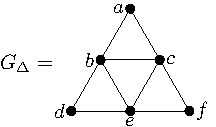
\includegraphics[height=\myMinHeight]{../../img/epsfromtikz/demo_graph}
%     \caption{}\label{fig:demo_graph:graph}
%   \end{subfigure}%
%   %
%   \hfill
%   \begin{subfigure}{0.3\linewidth}\centering
%     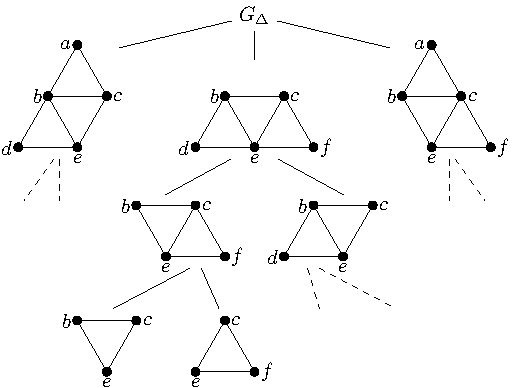
\includegraphics[height=\myMinHeight]{../../img/epsfromtikz/demo_graph_comdrp}
%     \caption{}\label{fig:demo_graph:comdrp}
%   \end{subfigure}%
%   %
%   \hfill
%   \begin{subfigure}{0.3\linewidth}\centering
%     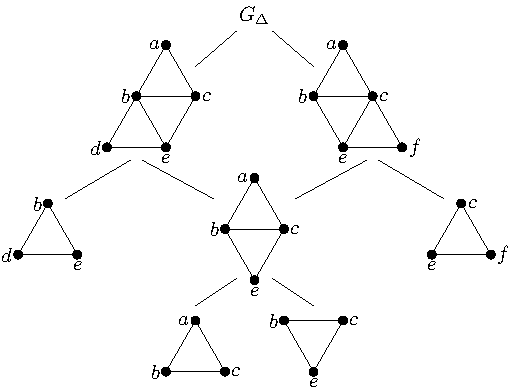
\includegraphics[height=\myMinHeight]{../../img/epsfromtikz/demo_graph_candrp}
%     \caption{}\label{fig:demo_graph:candrp}
%   \end{subfigure}%
%   %
%   \caption{(\ref{fig:demo_graph:graph}) A simple graph, $G_{\Delta}$, used to illustrate concepts throughout this and the next section. (\ref{fig:demo_graph:comdrp}) The complete DR-plan of $G_{\Delta}$, i.e.\ $ComDRP(G_{\Delta})$. Dashed lines indicate that the children repeat the same pattern as the others shown on this level. The children of triangles (3 edges) are omitted. (\ref{fig:demo_graph:candrp}) The canonical DR-plan of $G_{\Delta}$, which is optimal (see Section~\ref{sec:DRP}), i.e.\ $OptDRP(G_{\Delta})$. The children of triangles or omitted.}
%   \label{fig:demo_graph}
% \end{figure*}%

% \begin{figure*}\centering%
%   %
%   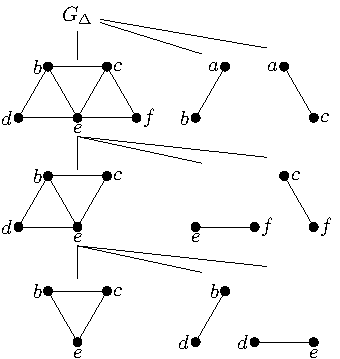
\includegraphics[width=0.3\linewidth]{../../img/epsfromtikz/demo_graph_candrp_seq}
%   \caption{The sequential canonical DR-plan of $G_{\Delta}$ from Figure~\ref{fig:demo_graph:graph}, which is optimal (as explained in the proof of Theorem~\ref{theorem:algo_complexity}). The children of the triangle are omitted. Compare to to the typical canonical DR-plan shown in Figure~\ref{fig:demo_graph:candrp}. Also, note that the bottom-left node, the triangle $bce$, is the intersection of the 3 children of $G_{\Delta}$ in $ComDRP(G_{\Delta})$, shown in Figure~\ref{fig:demo_graph:comdrp}.}
%   \label{fig:demo_graph:candrpseq}
% \end{figure*}%


To find the canonical DR-plan of an isostatic graph, we first need the following subroutine.

% \begin{theorem}\label{theorem:algo_find_wcvmps_complexity}
%     There exists an $O(|V|^2)$ time complexity algorithm to find the set of isostatic vertex-maximal proper subgraphs (the \dfn{clusters}) of an isostatic input graph.
% \end{theorem}

% \begin{proof}
%     Call the input graph $G=(V,E)$.
%     % If the input is not isostatic (i.e.\ does not satisfy $|E| = 2|V|-3$), run the component pebble game algorithm
%     Take an arbitrary edge $e\in E$. Run the component pebble game algorithm \cite{Jacobs:1997:PG} on the subgraph $G\setminus e$, which takes time $O(|V|^2)$. The output of this will be all of the maximal isostatic components of $G\setminus e$, which we will call the list of candidate-clusters, or $CC$. It will contain at most $|E|-1 = O(|V|)$ elements.

%     The next step is to isolate the set of true-clusters. Begin by initializing the list true-clusters, or $TC$, as an empty list. Then, for each subgraph $C\in CC$, run the \frontier\ algorithm \cite{hoffman2001decompositionII} \cite{lomonosov2004graph} on $C+e$ to find $D$ (which is the minimal isostatic subgraph containing $C+e$.) In case 1, where $D=G$, $C$ is removed from $CC$ and added to $TC$. In case 2, where $D\subsetneq G$, for all $H\in CC$ that are subgraphs of $D$, $H$ is removed from $CC$; then $D$ is added to $TC$. If every element in $CC$ results in case 1, add $e$ to $TC$. Thus, we do $O(|V|)$ work on $O(|V|)$ subgraphs for a total time of $O(|V|^2)$.
% \end{proof}

\begin{theorem}\label{theorem:algo_find_wcvmps_complexity}
    There exists an \complexityAllClustersV\ time complexity algorithm to find the set of isostatic vertex-maximal proper subgraphs (the \dfn{clusters}) of an isostatic input graph.
\end{theorem}

\begin{proof}
    Call the input graph $G=(V,E)$. Initialize the empty list of current-clusters, or $CC$. For each edge $e\in E$, run the component pebble game algorithm \cite{Jacobs:1997:PG} on the subgraph $G\setminus e$. The output of this will be all of the maximal isostatic components of $G\setminus e$, which we will call potential-clusters, or $PC$. Remove any element from $PC$ that is a subgraph of an element in $CC$, then remove any element from $CC$ that is a subgraph of an element in $PC$. Add all remaining elements of $PC$ to $CC$. Return $CC$ after running all edges.

    The time complexity is $O(|V|^3)$. For each edge, of which there are $O(|V|)$, we run the component pebble game, which takes $O(|V|^2)$, and then check its $PC$ against the $CC$, which also takes $O(|V|^2)$. This subgraph comparison can be done by labeling each edge in $E$ with a pointer to the element that contains it in $PC$ and $CC$ while running the component pebble games. Then, traverse edge set $E$ and check if the corresponding elements of $PC$ and $CC$ are subgraphs.
\end{proof}

\begin{figure*}\centering%
  %
  \includegraphics[width=0.3\linewidth]{../../img/svg/3xc2c3_candrp_seq}
  \caption{The sequential canonical DR-plan of $G_{demo}$ from Figure~\ref{fig:demo_graph:graph}, which is optimal (as explained in the proof of Theorem~\ref{theorem:algo_complexity}). The children of the triangle are omitted. Compare to to the typical canonical DR-plan shown in Figure~\ref{fig:demo_graph:candrp}. Also, note that the bottom-left node, the triangle, is the intersection of the 3 children of $G_{demo}$ in $ComDRP(G_{demo})$, shown in Figure~\ref{fig:demo_graph:comdrp}.}
  \label{fig:demo_graph:candrpseq}
\end{figure*}%

\begin{theorem}
\label{theorem:algo_complexity}
    There exists an \ComplexityCanDRPV\ algorithm to find a canonical DR-plan for an independent input graph.
\end{theorem}

\begin{proof}
    Call the input graph $G=(V,E)$. We will call the result of the algorithm $CanDRP(G)$.

    If $G$ is a single edge, return $G$.

    % Either $G$ is isostatic (i.e.\ satisfies $|E|=2|V|-3$)
    If $G$ is not isostatic (i.e.\ does not satisfy $|E|=2|V|-3$), run the component pebble game on $G$ to get the set of isostatic vertex-maximal subgraphs. Return the forest formed by recursively running $CanDRP$ on each element.

    If $G$ is isostatic, run the isostatic vertex-maximal proper subgraph detection algorithm (Theorem \ref{theorem:algo_find_wcvmps_complexity}) on $G$ to get what we call the list of clusters. This can be done in \complexityAllClustersV\ time. Choose two arbitrary clusters, called $C_1$ and $C_2$. If $C_1\cap C_2$ is trivial (a single vertex), recursively apply $CanDRP$ on all clusters and set the results as the children of $G$; return $G$. Else if $C_1\cap C_2$ is non-trivial (an isostatic subgraph), apply $CanDRP$ to $C_1$ (note that this choice is still arbitrary, any cluster will suffice) and $T$ (the underconstrained graph formed by $C\setminus C_1$ together with all incident edges and the associated vertices in $C$) and set the results as the children of $G$; return $G$.

    For the sake of increased clarity (and performance in implementation), we expand on the case of isostatic input with clusters that intersect non-trivially. Instead of immediate recursive application of $CanDRP$, we propose an equivalent method to first compute the decomposition down to $I=\bigcap_{k=1}^{N}{C_k}$. (The rationale and nomenclature is discussed in detail in the proof of Theorem \ref{theorem:main}.) Let $R_i= C\setminus C_i$; note that each $R_i$ is pairwise disjoint. Let $T_i$ be $R_i$ plus all incident edges; note that these edges are incident on vertices in $I$ and that $T_i$ is underconstrained. Let $S_i = C\setminus \bigcup_{j=1}^{i}{R_j}$. Set the children of $G$ as $S_1=C\setminus R_1=C_1$ and $CanDRP(T_1)$. Set the children of $S_1$ as $S_2=C\setminus (R_1\cup R_2)$ and $CanDRP(T_2)$. Etc. At step $N$, set the children of $S_{N-1}$ as $CanDRP(S_N)$ and $CanDRP(T_N)$. Thus we can avoid the $N$ recomputations of the isostatic components of $G$.

    We call this intermediate result of the algorithm the ``sequential'' canonical DR-plan. See Figure~\ref{fig:demo_graph:candrpseq} for an example. This plan is a tree, where each node is a distinct subgraph, each is smaller than its parent, and the leaves comprise the edge set of $G$. Therefore, the number of nodes in the tree is $O(|E|)$ which, for independent input graphs, is $O(|V|)$. The cluster finding algorithm is run on each internal node, resulting in an overall time complexity of \ComplexityCanDRPV.

    The sequential canonical DR-plan can then be used to find the canonical DR-plan in
    % sub-cubic
    sub-quartic
    time. Simply alter any subtree that is the result of non-trivial intersection in the obvious way (adding nodes for the clusters implied by the decomposition) to get the canonical DAG. Although, in practice, the sequential plan may be sufficient.
    %
    % \note In the best case, this can be $O(V^2)$ if the graph is a 2-tree
\end{proof}


% Note that in the case of each stage of decomposition resulting in trivial intersections, this algorithm can be run in time $O(|V|^3)$. We can find all clusters in time $O(|V|^2)$, because we only have to look at a constant number of edges. Take two arbitrary edges to get the two sets of potential-clusters, $PC_1$ and $PC_2$.



% \begin{proof}
%     Choose an arbitrary ordering of the edges, such that $e_i$ is the $i^\text{th}$ edge in the sequence.

%     Run component pebble game on each edge to get the map $M$ that takes an edge, $e$, and returns a set of subgraphs that are the output of the component pebble game on $G\setminus e$. On each run of the pebble game, also attach a pointer to each edge that points to the subgraph containing the edge.
%     Call this map $P$, where $P(i, j)$ (which is not defined where $i=j$) returns a pointer to the element containing $e_i$ from $M(e_j)$.
%     This is $O(|V|^3)$.

%     Dropping an edge will never result in some other edge being in some new cluster, the other edge will only ever be in a subset of its true cluster. Therefore, we can look at each edge in $E$ and find the proper maximal subgraph containing it by following all the cluster pointers and comparing the cardinality of the vertex sets, taking the largest. This can be done in $O(|V|^2)$. Save any subgraph found in this manner.
%     HAVE TO CHECK FOR DUPLICATES... CAN BE ROLLED INTO NEXT STEP, DIFFERENT BASED ON INTERSECTION TYPE. JUST DO AN EDGE FROM THE COMPLEMENT ($G\setminus C$) SECOND.

%     Now check the intersections between clusters (pick an arbitrary two).

%     In the case of trivial intersections, all of the found clusters will be edge-disjoint.
%     For each cluster $C$, take the submatrix of $P$ only on the intersections of elements in $C$. That is, if $C$ contains $i$ and $j$, keep element $P(i,j)$. Delete any element in $M$ whose pointer is lost from $P$ after this operation.
%     % For each edge $e_i$, for every edge $e_j$ not in the cluster to which $e_i$ belongs, delete $P(i, j)$ and the element it points to in $M(e_j)$ (if it isn't already deleted).
%     This can be done in $O(|V|^2)$ time.
%     The result will be a new $P$ and $M$ for each cluster, containing only the edges in the cluster. Furthermore, all clusters from this stage will be removed from $M(e_i)$ (for all $i$).
%     % Divide the edges into sets based on their containing cluster (one edge is contained in only one cluster) and repeat the previous step.
%     Recursively run the algorithm on these clusters, but we can now skip the first step, avoiding $O(|V|^3)$ work at each node... So with an initial step of $O(|V|^3)$ and then $O(|V|^2)$ work at $O(|V|)$ nodes we get an overall complexity of $O(|V|^3)$.

%     In the case of isostatic intersections, you will find 2 clusters (the one with the most vertices, $C_1$, and the largest one containing the vertex set omitted from the first, $C_2$). You will also need to be careful of different clusters with the same size (just be aware it might happen, shouldn't affect anything, we'll want them later). Go to an arbitrary edge not in $C_1$. Look at the clusters containing the edge with the largest cardinality. The largest will be $C_2$, ignore it. Keep going to the next largest, adding it to the list of found clusters if it has an isostatic intersection with the $C_1$. This will take $O(|V|^2)$. Now we have all of the isostatic vertex-maximal proper subgraphs, which we call $C_1, C_2, \ldots , C_N$. Compute the intersection of all of these, which we call the ``core'' or $I$. Let $R_i = G\setminus C_i$.

%     Choose an arbitrary edge $e\in I$. Take the set $M(e)$, remove all elements that are subgraphs of $I$. Of the remainder, the elements that are subgraphs of $R_i$ are the first level of decomposition of $R_i$ and we call this subset $T_i$. Now we are ready to build the ``sequential'' canonical DR-plan of $G$ down to node $I$.

%     Set the children of $G$ as $S_1=C\setminus R_1=C_1$ and the elements of $T_1$. Set the children of $S_1$ as $S_2=C\setminus (R_1\cup R_2)$ and the elements of $T_2$. Etc. At step $N$, set the children of $S_{N-1}$ as $S_N=I$ and the elements of $T_N$.

%     For node $I$ and each element of $T_1, T_2, \ldots , T_N$ in the DR-plan, get the submatrix of $P$ using the edges of the subgraph in the node, and update $M$ accordingly.
%     % For each edge $e_i$ in the core, for every edge $e_j$ not in the core, delete $P(e_i, j)$ and the element it points to in $M(e_j)$ (if it isn't already deleted).

%     The sequential canonical DR-plan can then be used to find the canonical DR-plan in
%     sub-cubic
%     % sub-quartic
%     time. Simply alter any subtree that is the result of non-trivial intersection in the obvious way (adding nodes for the clusters implied by the decomposition) to get the canonical DAG. Although, in practice, the sequential plan may be sufficient.
% \end{proof}

First, we remind the reader of the component pebble game~\cite{Jacobs:1997:PG}. Given an independent input graph $G$ with vertex weight 2 and edge weight 1, the output will be all of the 2D maximal isostatic subgraphs. We will denote this algorithm with $COMPONENTS(G)$. For independent input, this runs in time $O(|V|^2)$.

We also introduce the term \dfn{clusters} of graph $G$ to refer to the set of isostatic vertex-maximal proper subgraphs of $G$.

Next, we define an operation called \dfn{modularization}. The function $MZ(M, I)$ takes a square matrix $M$ and a set of indices $I$ and returns $(M', A)$. $M'$ is the square matrix formed by keeping all elements $M_{ij}$ if $i,j\in I$. $A$ is the set of elements $M_{ij}$ and $M_{ji}$ where $i\in I$ and $j\notin I$.
% This operation takes $O(|I|^2)$.

% Next, we make the observation that dropping an edge will only cause other edges in the graph to be in components (as found by pebble games) that are subgraphs of their cluster ()

% Consider dropping edge $e_i$ and looking at the effect on $e_j$. In the case that all clusters intersect trivially, no edge is in multiple clusters. Therefore, $e_i$ could come from a different cluster than $e_j$, in which case dropping $e_i$ only affects its own cluster. Or $e_i$ could come from the same cluster as $e_j$, in which case all other clusters are found as components, but additionally edge-disjoint subgraphs of this cluster will be found as components.
% In the case that clusters intersect non-trivially, edges do com from multiple clusters.

\begin{proof}
    %% INITIALIZATION
    Let the input be $G=(E,V)$. If the input is an edge, terminate. If the input is not isostatic, set the roots of the forest as $COMPONENTS(G)$ then recursively call the algorithm on each root. Otherwise, do the following.

    Choose an arbitrary ordering of the edges, such that $e_i$ is the $i^\text{th}$ edge in the sequence.
    Initialize a map $M$ and a map $P$. For each $i$, set $M(e_i)=COMPONENTS(G\setminus e_i)$ and, for all $j\neq i$, set $P(i,j)$ as a pointer to the element in $M(e_i)$ whose subgraph contains $e_j$. This initialization takes time $O(|V|^3)$.


    %% STEP 1: Find the clusters
    % Choose some $i\leq |E|$, then find the
    Now we want to find the clusters of $G$.
    For each $i$, if we have not already found a cluster containing $e_i$, then find the $j$ such that $P(j,i)$ points to the component with the largest cardinality and add it to the list of clusters. This takes time $O(|V|^2)$. In the case that the clusters intersect trivially, we will find all of the clusters. In the case that they intersect non-trivially, we will find exactly two clusters. We will return to the latter case after continuing the proof for the former.

    %% STEP 2a: Trivial intersections
    In the case of trivial intersections, all of the found clusters will be edge-disjoint. For each cluster edge set $C_i$, compute $MZ(P, C_i)=(P_i, A_i)$. For element in each $A_i$, delete the component it points to in $M$. This can be done in $O(|V|^2)$ time.
    Note that, for any $i$, $M(e_i)$ contained only subgraphs of the cluster containing $e_i$ and the other clusters. By doing the deletions, we have removed all of the clusters found in this stage. This means $M$ can now be broken into an $M_i$ for each $C_i$, where $M_i$ contains only proper subgraphs of $C_i$. Now the algorithm can be run recursively on each $C_i$, while avoiding the recomputation of $M$ and $P$ by using the $M_i$ and $P_i$ we found.

    %% STEP 2b: Non-trivial intersections
    In the case of non-trivial intersections, we have only found 2 clusters (the one with the most vertices, $C_1$, and the largest one containing the vertex set omitted from the first, $C_2$) and we need to find the remainder. Go to an arbitrary edge $e_i\notin C_1$. For all $j\neq i$, if the component pointed to by $P(j,i)$ intersects non-trivially with $C_1$ add it to the list of clusters (ignore duplicates). This will take $O(|V|^2)$. Now we have all of the isostatic vertex-maximal proper subgraphs, which we call $C_1, C_2, \ldots , C_N$. Let $I=\bigcap_{k=1}^{N}{C_k}$. Let $R_i = G\setminus C_i$.
    Let $T_i = COMPONENTS(R_i)$. All of these can be computed in $O(|V|^2)$.

    % Choose an arbitrary edge $e\in I$. Take the set $A=M(e)$, remove all elements from $A$ that are subgraphs of $I$. For each $R_i$, find the set $T_i$ which contains the elements of $A$ that are subgraphs of $R_i$. Note that $T_i=COMPONENTS(R_i)$, and will be the first level of decomposition of $R_i$ since it is underconstrained.
    % COULD WE JUST RUN $COMPONENTS$???

    Now we build the ``sequential'' canonical DR-plan of $G$ down to node $I$.
    Set the children of $G$ as $S_1=C\setminus R_1=C_1$ and the elements of $T_1$. Set the children of $S_1$ as $S_2=C\setminus (R_1\cup R_2)$ and the elements of $T_2$. Etc. At step $N$, set the children of $S_{N-1}$ as $S_N=I$ and the elements of $T_N$.
    For each node $N$ of the DR-plan in the set $\{I\}\cup T_1\cup T_2\cup \cdots\cup T_N$, compute $MZ(P, N)=(P', A')$ and update $M$ by deleting all elements pointed to by $A'$. Then, for each $N$, run the algorithm recursively on (avoiding recomputation of $M$ and $P$).
    % For node $I$ and each element of $T_1, T_2, \ldots , T_N$ in the DR-plan, compute $MZ(P, \cdot)$, update $M$ in the same fashion as above, and run the algorithm recursively on $(\cdot)$ (avoiding recomputation of $M$ and $P$).

    %% Proof of complexity
    The decomposition will ultimately terminate as a tree with $|E|$ leaves, each containing a unique edge. With an initial step of $O(|V|^3)$ and then $O(|V|^2)$ work at $O(|V|)$ nodes we get an overall complexity of $O(|V|^3)$.

    The sequential canonical DR-plan can then be used to find the canonical DR-plan in
    sub-cubic
    % sub-quartic
    time. Simply alter any subtree that is the result of non-trivial intersection in the obvious way (adding nodes for the clusters implied by the decomposition) to get the canonical DAG. Although, in practice, the sequential plan may be sufficient.
\end{proof}











% \begin{proof}
% The first step of the algorithm is finding the isostatic vertex-maximal proper subgraphs of the input isostatic graph $G$. Do this by first dropping arbitrary edge $e$ from the edge set and running the pebble game algorithm \cite{Jacobs:1997:PG} on this subgraph, which is $O(|V|^2)$. The output of this will be a list of component-candidates. Then run the \frontier\ algorithm \cite{hoffman2001decompositionII} \cite{lomonosov2004graph} ($O(|V|)$) on each candidate along with edge $e$, which will find the minimal subgraph $D$ that contains the candidate and $e$. If $D=G$, move $D$ to the true-cluster list and remove the candidate from the candidate-component list. If $D\subsetneq G$, check the union of $D$ with the all items in the true-cluster list; if the union is isostatic, halt and output just these two components as children. Otherwise, remove all candidates that are subgraphs of $D$ from the candidate-component list and add $D$. Continue with the next candidate. If you exhaust the candidates, output the entire true-cluster list.

% %on the children
% This is run recursively on each node. If you use dynamic programming to store the decompositions of each component, it prevents repetition of work (done by using the DAG representation of the DR-plan). In this case you will have to do work on no more than $O(|V|)$ nodes that get smaller at each level.

% Thus, the running time is at most $O(|V|^3)$. \todo{does this amortize correctly?}

% It's a tree in only trivial case -> O(V), always order of leaves
% If its isostatic intersection, we do the sequential extension,intersections only done once.

% inductively. The number of nodes at this level will e more than the total. Number of leaves (terminals for dag) is at most the number of edges

% \end{proof}

% \begin{proof}
% The first step of the algorithm to find an optimal DR-plan is the most difficult --- to find the wellconstrained vertex-maximal proper subgraphs of the input wellconstrained graph. There are two approaches: (1) the bottom-up approach, using the \frontier\ algorithm \cite{Oung:2001:FFE:376957.376995} to grow these components from single vertices; and (2) the top-down approach, using the pebble game algorithm \cite{Jacobs:1997:PG} on each node and taking the largest components that are not subgraphs of any larger ones. After the subgraphs have been found, it is a straightforward application of the theory. If the intersection of any two of the subgraphs is wellconstrained, then take those two to be children of the graph. Otherwise, all the subgraphs are the children. Apply recursively to the children. This naturally terminates when you reach trivial subgraphs. The complexity of this depends on the algorithm for finding children (both are polynomial) and the depth of the plan (the deeper the plan, i.e.\ the smaller the max fan-in, the longer the running time). \todo{Think more about complexity.}
% \end{proof}

















While the canonical DR-plan is clear conceptually, it is difficult to reason with directly in the design and analysis of algorithms. Therefore, we introduce the following modification to get a similar but more useful structure.

\begin{figure*}\centering%
  %
  \includegraphics[width=0.3\linewidth]{../../img/svg/3xc2c3_candrp_seq}
  \caption{The sequential canonical DR-plan of $G_{demo}$ from Figure~\ref{fig:demo_graph:graph}, which is optimal (as explained in the proof of Theorem~\ref{theorem:algo_complexity}). The children of the triangle are omitted. Compare to to the typical canonical DR-plan shown in Figure~\ref{fig:demo_graph:candrp}. Also, note that the bottom-left node, the triangle, is the intersection of the 3 children of $G_{demo}$ in $ComDRP(G_{demo})$, shown in Figure~\ref{fig:demo_graph:comdrp}.}
  \label{fig:demo_graph:candrpseq}
\end{figure*}%


\begin{definition}
    A \dfn{sequential} canonical DR-plan (or simply sequential DR-plan) is a canonical DR-plan with the following modification:

    In the case that a node has isostatic vertex-maximal proper subgraphs (or clusters) that intersect non-trivially.
    we construct a \dfn{sequential extension} in the following manner.
    %
    Let the current node be $G$.
    Let the $N$ clusters be $C_1, C_2, \ldots, C_N$.
    Let the \dfn{core} be $I=\bigcap_{k=1}^{N}{C_k}$.
    Let the $N$ \dfn{appendages} be $R_i = G\setminus C_i$.
    %
    Choose arbitrary appendage $R_i$ and set the children of $G$ as $I\cup \bigcup_{k=1}^{i}{R_k}\cup \bigcup_{k=i}^{N}{R_k}$ and the clusters of $R_i$. Construct the sequential canonical DR-plan of each child.
\end{definition}

See Figure~\ref{fig:demo_graph:candrpseq} for an example. Note the pattern will continue for $N$ levels, where $N$ is the number of appendages. At the top is $G$, the core with all appendages; at the next level, the children are the core with all but one appendage and the clusters of the removed appendage; at the next level, it has the core with all but two appendages and the clusters of the appendage removed second; etc.; at the bottom level is the core.

\begin{observation}
    A sequential canonical DR-plan of independent graph $G=(V,E)$ is a tree with $O(|V|)$ nodes.
\end{observation}

\begin{observation}
    A sequential canonical DR-plan of an independent graph is optimal.
\end{observation}

\begin{proof}
    A sequential DR-plan behaves the same as a canonical DR-plan in the case of a node whose clusters have trivial intersections.
    In a regular canonical DR-plan, at a node with $N$ clusters that intersect non-trivially, there is fan-in of 2 until level $N$. At level $N-1$, there are $N$ distinct nodes, one for each appendage together with the core. The children of these nodes are the core and the clusters of the corresponding appendage. Thus, the maximum fan-in over this part of the canonical DR-plan is one plus the maximum number of clusters in an appendage. By construction, this is exactly the maximum fan-in of a sequential extension.
\end{proof}

\begin{observation}\label{obs:seq-to-reg-canonical}
    Given a sequential canonical DR-plan of an independent graph $G=(V,E)$, a canonical DR-plan can be found in time $O(|V|^3)$.
\end{observation}

\begin{proof}
    In the case of a node whose children intersect trivially, nothing needs to be done.
    In the case of non-trivial intersections, we will need to construct the canonical DR-plan subtree from the sequential extension.

    At such a node $G$ with $N$ clusters, we will have to build $\sum_{i=1}^N{i}=O(N^2)$ new nodes. For convenience, $C_{[i,j]}$ will represent the core plus appendages $i$ through $j$. We set the children of $G$ as $C_{[0,N-1]}$ and $C_{[1,N]}$. The children of $C_{[0,N-1]}$ are set as $C_{[0,N-2]}$ and $C_{[1,N-1]}$. The children of $C_{[1,N]}$ are set as $C_{[1,N-1]}$ (not unique) and $C_{[2,N]}$. This pattern continues for $N$ levels, with level $i$ containing $i$ unique nodes.

    Since there are at most $O(|V|)$ nodes with $O(|V|)$ clusters that need this treatment, the complexity is $O(|V|^3)$.
\end{proof}


Before discussing the algorithm, we remind the reader of the component pebble game~\cite{Jacobs:1997:PG}. Given an independent input graph $G$ with vertex weight 2 and edge weight 1, the output will be all of the 2D maximal isostatic subgraphs (the components). We will denote this algorithm with $\components{G}$. For independent input, this runs in time $O(|V|^2)$.

The algorithm for finding the sequential DR-plan is going to rely on the observation that the set of $\components{G\setminus e}$ over all $e\in E$ will (essentially) encompass all the nodes of the sequential DR-plan for $G$, with minor caveats that we will explain later.

\begin{lemma}\label{lemma:seq-nontriv-Gtoe}
    When the intersections of clusters are trivial at all nodes in the (sequential) canonical DR-plan, then the set $\components{G\setminus e}$ will contain all of the siblings in the path from $G$ to $e$.
\end{lemma}

\begin{proof}
    The sequential and canonical DR-plans are identical in this case. Suppose $G$ has $N$ trivially intersecting components, and $e$ is in component $C_i$. Removing edge $e$ will leave all components besides $C_i$ intact, thus they will be isostatic components in $G\setminus e$ and will be in the set. Therefore, $\components{G\setminus e}$ contains
    % $C_1, \ldots, C_{i-1}, C_{i+1}, \ldots, C_N$
    all clusters besides $C_i$
    and the set $\components{C_i\setminus e}$. By induction, the proof is complete.
\end{proof}

\begin{lemma}\label{lemma:seq-Gtoe}
    In the (sequential) canonical DR-plan, the set $\components{G\setminus e}$ will contain all of the siblings in the path from $G$ to $e$ excluding the following: in the case of a node whose $N$ clusters have non-trivial intersections, those nodes that contain the core plus any $i$ appendages where $0\leq i<N-1$.
\end{lemma}

\begin{proof}
    By Lemma~\ref{lemma:seq-nontriv-Gtoe}, this is true for trivial intersections. For non-trivial intersections, consider an edge $e$ that comes from appendage $R_i$. Then $\components{G\setminus e}$ will contain the element `core plus all appendages but $R_i$' and the set $\components{R_i\setminus e}$, so the statement is true. Now, consider an edge $e$ that comes from $I$, the core. Then $\components{G\setminus e}$ will contain $\components{R_i}$ for all appendages $R_i$ and $\components{I\setminus e}$.
\end{proof}

Note that in the sequential DR-plan, the number of missing nodes is at worst $O(|V|^2)$. There can be as many as $O(|V|)$ nodes with non-trivial intersections on $O(|V|)$ clusters, each cluster contributing one appendage and one missing node (excluding the first in the sequential extension).

\begin{theorem}\label{theorem:algo_complexity}
    There exists an \ComplexityCanDRPV\ *** algorithm to find a canonical DR-plan for an independent graph.
\end{theorem}

\begin{proof}
    Let the input graph be $G=(V,E)$. Begin by computing $\components{G\setminus e}$ for all $e\in E$ in $O(|V|^3)$. By Lemmas~\ref{lemma:seq-nontriv-Gtoe} and \ref{lemma:seq-Gtoe}, this will contain all but a select group of nodes in the sequential DR-plan. Because the sequential DR-plan is a tree whose leaves are unique edges, there are $O(|V|)$ nodes. At each node, if the children can be determined in $O(|V|^2)$, the sequential DR-plan can be found in time $O(|V|^3)$ as a whole. By Observation~\ref{obs:seq-to-reg-canonical}, this would mean a canonical DR-plan can be found in $O(|V|^3)$.

    First, we find the children. For each edge $e_i$, find the largest component from all $\components{G\setminus e_j}$ containing $e_i$. This is a cluster containing $e_i$ (in the case of trivial intersections, it is the only cluster containing $e_i$).

    If the clusters intersect trivially, every cluster $C_1, C_2, \ldots, C_N$ will be found this way. For each cluster $C_i$, for each edge $e_j\in C_i$, compute $\components{C_i\setminus e_j}$ by removing the other clusters from $\components{G\setminus e_j}$; set $C_i$ as a child of $G$ and run the algorithm recursively without the $O(|V|^3)$ time recomputation of the components.

    If the clusters intersect non-trivially, exactly two clusters will be found this way. Cluster $C_1$ will be the largest cluster overall and $C_2$ will be the largest cluster that contains appendage $R_1$. To find the remaining clusters, choose an arbitrary edge $e_i\in R_1$, for each edge $e_j\neq e_i$, if the component containing $e_i$ in $\components{G\setminus e_j}$ intersects non-trivially with $C_1$ then it is a cluster and is added to the list, otherwise $e_j$ came from the core. Once all clusters are found, the core and the appendages can be determined, and the sequential extension from $G$ can be computed. The incomplete children will be the sets $\components{R_i}$ for all appendage $R_i$ and the node containing the core. Before recursion, for each incomplete child $P$, for each $e\in P$, find $\components{P\setminus e}$ by removing the appropriate elements from $\components{G\setminus e}$.
\end{proof}


